%%%%%%%%%%%%%%%%%%%%%%%%%%%%%%%%%%%%%%%%%
% Beamer Presentation
% LaTeX Template
% Version 2.0 (March 8, 2022)
%
%cmd Befehl: pdflatex -shell-escape presentation.tex
%
% This template originates from:
% https://www.LaTeXTemplates.com
%
% Author:
% Vel (vel@latextemplates.com)
%
% License:
% CC BY-NC-SA 4.0 (https://creativecommons.org/licenses/by-nc-sa/4.0/)
%
%%%%%%%%%%%%%%%%%%%%%%%%%%%%%%%%%%%%%%%%%

%----------------------------------------------------------------------------------------
%	PACKAGES AND OTHER DOCUMENT CONFIGURATIONS
%----------------------------------------------------------------------------------------

\documentclass[
	11pt, % Set the default font size, options include: 8pt, 9pt, 10pt, 11pt, 12pt, 14pt, 17pt, 20pt
	%t, % Uncomment to vertically align all slide content to the top of the slide, rather than the default centered
	aspectratio=169, % Uncomment to set the aspect ratio to a 16:9 ratio which matches the aspect ratio of 1080p and 4K screens and projectors
]{beamer}

\graphicspath{{Images/}{./}} % Specifies where to look for included images (trailing slash required)

\usepackage{booktabs} % Allows the use of \toprule, \midrule and \bottomrule for better rules in tables

%----------------------------------------------------------------------------------------
%	SELECT LAYOUT THEME
%----------------------------------------------------------------------------------------

% Beamer comes with a number of default layout themes which change the colors and layouts of slides. Below is a list of all themes available, uncomment each in turn to see what they look like.

%\usetheme{default}
%\usetheme{AnnArbor}
%\usetheme{Antibes}
%\usetheme{Bergen}
%\usetheme{Berkeley}
%\usetheme{Berlin}
%\usetheme{Boadilla}
%\usetheme{CambridgeUS}
%\usetheme{Copenhagen}
%\usetheme{Darmstadt}
%\usetheme{Dresden}
%\usetheme{Frankfurt}
%\usetheme{Goettingen}
%\usetheme{Hannover}
%\usetheme{Ilmenau}
%\usetheme{JuanLesPins}
%\usetheme{Luebeck}
\usetheme{Madrid}
%\usetheme{Malmoe}
%\usetheme{Marburg}
%\usetheme{Montpellier}
%\usetheme{PaloAlto}
%\usetheme{Pittsburgh}
%\usetheme{Rochester}
%\usetheme{Singapore}
%\usetheme{Szeged}
%\usetheme{Warsaw}

%----------------------------------------------------------------------------------------
%	SELECT COLOR THEME
%----------------------------------------------------------------------------------------

% Beamer comes with a number of color themes that can be applied to any layout theme to change its colors. Uncomment each of these in turn to see how they change the colors of your selected layout theme.

%\usecolortheme{albatross}
%\usecolortheme{beaver}
%\usecolortheme{beetle}
%\usecolortheme{crane}
%\usecolortheme{dolphin}
%\usecolortheme{dove}
%\usecolortheme{fly}
%\usecolortheme{lily}
%\usecolortheme{monarca}
%\usecolortheme{seagull}
%\usecolortheme{seahorse}
%\usecolortheme{spruce}
%\usecolortheme{whale}
%\usecolortheme{wolverine}

%----------------------------------------------------------------------------------------
%	SELECT FONT THEME & FONTS
%----------------------------------------------------------------------------------------

% Beamer comes with several font themes to easily change the fonts used in various parts of the presentation. Review the comments beside each one to decide if you would like to use it. Note that additional options can be specified for several of these font themes, consult the beamer documentation for more information.

%\usefonttheme{default} % Typeset using the default sans serif font
\usefonttheme{serif} % Typeset using the default serif font (make sure a sans font isn't being set as the default font if you use this option!)
%\usefonttheme{structurebold} % Typeset important structure text (titles, headlines, footlines, sidebar, etc) in bold
%\usefonttheme{structureitalicserif} % Typeset important structure text (titles, headlines, footlines, sidebar, etc) in italic serif
%\usefonttheme{structuresmallcapsserif} % Typeset important structure text (titles, headlines, footlines, sidebar, etc) in small caps serif

%------------------------------------------------

%\usepackage{mathptmx} % Use the Times font for serif text
\usepackage{palatino} % Use the Palatino font for serif text
\usepackage{stackengine}
%\usepackage{helvet} % Use the Helvetica font for sans serif text
\usepackage[default]{opensans} % Use the Open Sans font for sans serif text
%\usepackage[default]{FiraSans} % Use the Fira Sans font for sans serif text
%\usepackage[default]{lato} % Use the Lato font for sans serif text
\usepackage{amsmath,amsfonts,amssymb}
%\usepackage[german]{babel}
\usepackage[ngerman]{babel}
\usepackage{minted}
\usepackage{listings}
\usepackage{datetime}
\newdateformat{myformat}{\THEDAY{. }\monthname[\THEMONTH], \THEYEAR}
%----------------------------------------------------------------------------------------
%	SELECT INNER THEME
%----------------------------------------------------------------------------------------

% Inner themes change the styling of internal slide elements, for example: bullet points, blocks, bibliography entries, title pages, theorems, etc. Uncomment each theme in turn to see what changes it makes to your presentation.

%\useinnertheme{default}
\useinnertheme{circles}
%\useinnertheme{rectangles}
%\useinnertheme{rounded}
%\useinnertheme{inmargin}

%----------------------------------------------------------------------------------------
%	SELECT OUTER THEME
%----------------------------------------------------------------------------------------

% Outer themes change the overall layout of slides, such as: header and footer lines, sidebars and slide titles. Uncomment each theme in turn to see what changes it makes to your presentation.

%\useoutertheme{default}
%\useoutertheme{infolines}
%\useoutertheme{miniframes}
%\useoutertheme{smoothbars}
%\useoutertheme{sidebar}
%\useoutertheme{split}
%\useoutertheme{shadow}
%\useoutertheme{tree}
%\useoutertheme{smoothtree}

%\setbeamertemplate{footline} % Uncomment this line to remove the footer line in all slides
%\setbeamertemplate{footline}[page number] % Uncomment this line to replace the footer line in all slides with a simple slide count

%\setbeamertemplate{navigation symbols}{} % Uncomment this line to remove the navigation symbols from the bottom of all slides

%----------------------------------------------------------------------------------------
%	PRESENTATION INFORMATION
%----------------------------------------------------------------------------------------

\title[NSG]{Navier-Stokes Gleichungen} % The short title in the optional parameter appears at the bottom of every slide, the full title in the main parameter is only on the title page

%\subtitle{Optional Subtitle} % Presentation subtitle, remove this command if a subtitle isn't required

\author[Jannik Schrempp\and Hendrik Klemm]{}%{Capt. James Cook \and Roald Amundsen} % Presenter name(s), the optional parameter can contain a shortened version to appear on the bottom of every slide, while the main parameter will appear on the title slide

\institute[]{University of Stuttgart IAG} %\\ %\smallskip \textit{james@LaTeXTemplates.com}} % Your institution, the optional parameter can be used for the institution shorthand and will appear on the bottom of every slide after author names, while the required parameter is used on the title slide and can include your email address or additional information on separate lines

\date[\myformat\today]{Studentenvortrag \\ \myformat\today} % Presentation date or conference/meeting name, the optional parameter can contain a shortened version to appear on the bottom of every slide, while the required parameter value is output to the title slide

%----------------------------------------------------------------------------------------
\titlegraphic{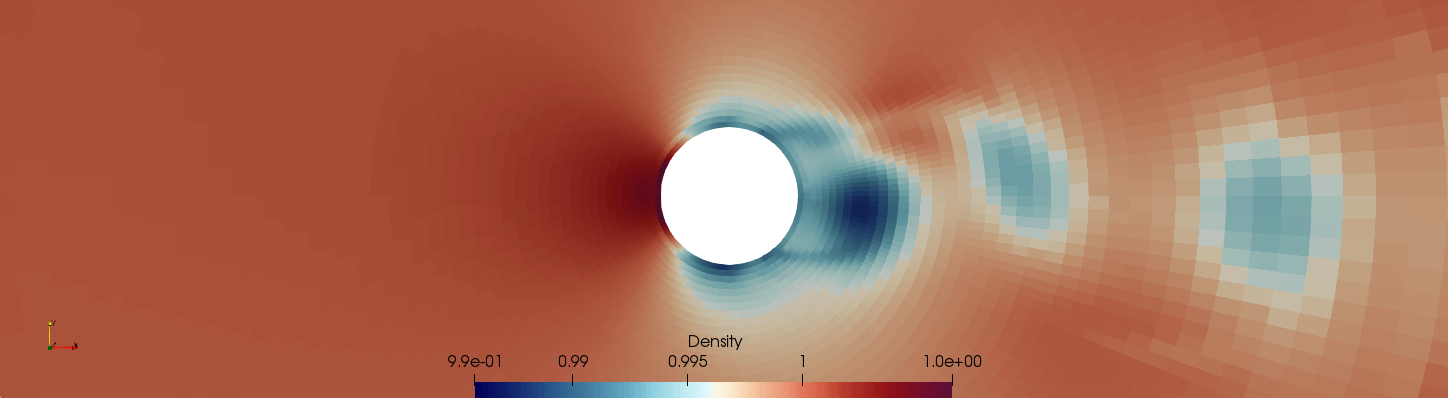
\includegraphics[width=1\textwidth,height=0.5\textheight]{Title.png}}
\begin{document}
\newcommand\barbelow[1]{\stackunder[1.2pt]{$#1$}{\rule{.8ex}{.075ex}}}
%----------------------------------------------------------------------------------------
%	TITLE SLIDE
%----------------------------------------------------------------------------------------

\begin{frame}
	% \vspace{-2cm}
	% \begin{figure}
	% 	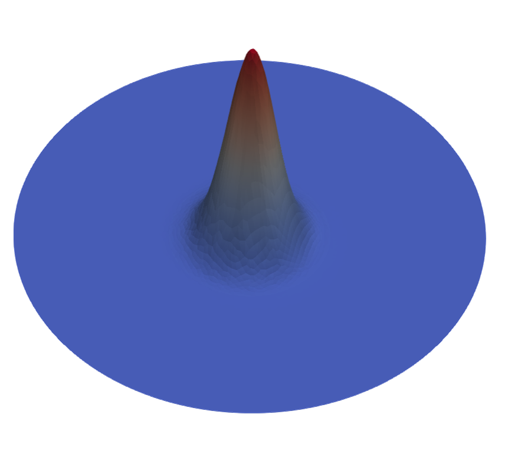
\includegraphics[width=0.5\linewidth]{title_Gausspuls.png}
		
	% \end{figure}
	\titlepage % Output the title slide, automatically created using the text entered in the PRESENTATION INFORMATION block above

\end{frame}

%----------------------------------------------------------------------------------------
%	TABLE OF CONTENTS SLIDE
%----------------------------------------------------------------------------------------

% The table of contents outputs the sections and subsections that appear in your presentation, specified with the standard \section and \subsection commands. You may either display all sections and subsections on one slide with \tableofcontents, or display each section at a time on subsequent slides with \tableofcontents[pausesections]. The latter is useful if you want to step through each section and mention what you will discuss.

\begin{frame}
	\frametitle{Überblick} % Slide title, remove this command for no title
	
	\tableofcontents % Output the table of contents (all sections on one slide)
	%\tableofcontents[pausesections] % Output the table of contents (break sections up across separate slides)
\end{frame}

%----------------------------------------------------------------------------------------
%	PRESENTATION BODY SLIDES
%----------------------------------------------------------------------------------------

\section{Grundlagen} % Sections are added in order to organize your presentation into discrete blocks, all sections and subsections are automatically output to the table of contents as an overview of the talk but NOT output in the presentation as separate slides

%------------------------------------------------
\subsection{Navier-Stokes Gleichungen}


\begin{frame}
	\frametitle{Navier-Stokes Gleichungen}
	Eulergleichungen sind Vereinfachung der Navier-Stokes Gleichungen für $\mathrm{Re} \rightarrow \infty$\\
	\begin{equation}
	\begin{split}
		\rho_t + \nabla\cdot (\rho v) &= 0\\
		(\rho v)_t + \nabla\cdot ((\rho v)\circ v) + \nabla p &= \textcolor{red}{\nabla \tau} \\
		e_t + \nabla \cdot (v(e+p)) &= \textcolor{red}{\nabla \cdot (\tau \cdot v) - \nabla \cdot q}  \\
	\end{split}
\end{equation}



	

	Zusätzliche Terme:\\
	Reibungstensor $\tau = \mu (\nabla v + (\nabla v)^T) - \frac{2}{3}\mu (\nabla \cdot v)$\\
	Wärmeleitung $q = -\frac{c_p\mu}{Pr}\nabla T$\\
	\newline

	Analog zu den Eulergleichungen können auch die Navier-Stokes-Gleichungen in die Flussformulierung gebracht werden.
	\begin{equation}
		\mathrm{U}_t + \nabla \cdot \mathbb{F}^C (\mathrm{U}) = \nabla \cdot \mathbb{F}^D(\mathrm{U}, \nabla \mathrm{U})
	\end{equation}




	% das v gefällt mir nicht, andere schriftart
\end{frame}

\begin{frame}
	\frametitle{Navier-Stokes Flüsse}
	\begin{columns}
	\column{0.5\textwidth}
	konvektive Flüsse:
	\begin{itemize}
		\item hyperbolisch
		\item Transport von Information
	\end{itemize}

	\begin{figure}
			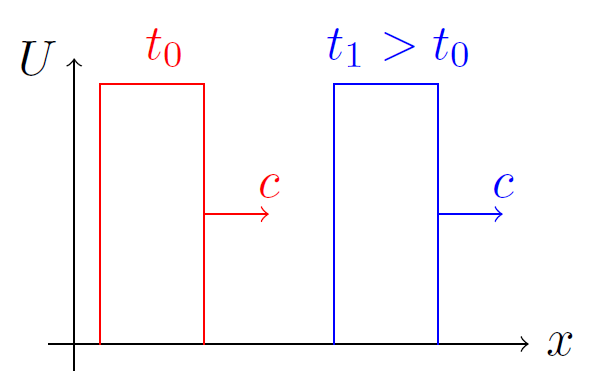
\includegraphics[width=0.8\linewidth]{konvekitv.png}
	\end{figure}
	\column{0.5\textwidth}
	viskose Flüsse:
	\begin{itemize}
		\item parabolisch
		\item Dissipation und Wärmeleitung
	\end{itemize}

	\begin{figure}
			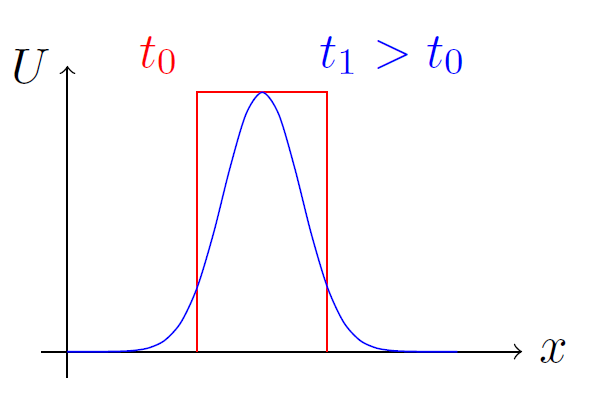
\includegraphics[width=0.8\linewidth]{Viskos.png}
			%\caption{Gausspuls auf kartesischem Gitter (oben) und unstrukturiertem kreisförmigem Gitter (unten)}
		\end{figure}
	\end{columns}
\end{frame}

\begin{frame}
	\frametitle{Viskoste Flüsse}
	\begin{center}
		\begin{figure}
			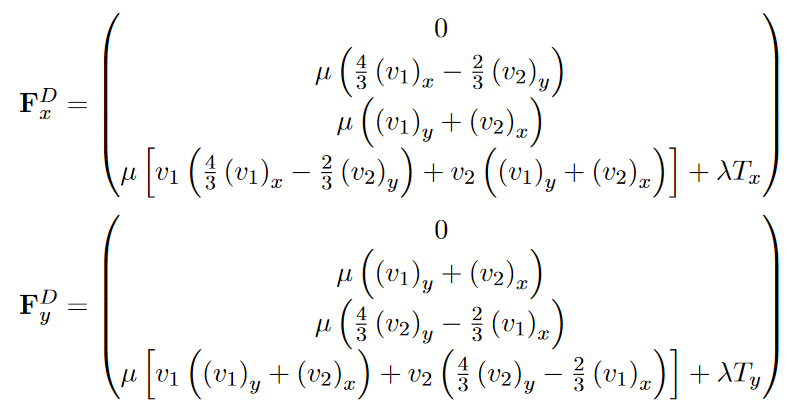
\includegraphics[width=0.8\linewidth]{visc_fluesse.png}
			%\caption{Gausspuls auf kartesischem Gitter (oben) und unstrukturiertem kreisförmigem Gitter (unten)}
		\end{figure}
	\end{center}
% Hier sehen wir, dass wir zusätzlich zu den Größen auch die Ableitungen brauchen. Wie kommen wir also an die Ableitungen? -> Nächste Folie
\end{frame}




\subsection{viskose Zeitschrittbedingung}
\begin{frame}
	\frametitle{Viskose Zeitschrittbedingung}
	Parabolischer Charakter der Reibungsterme beeinflussen die Stabilität des numerischen Verfahrens stark
	$\Rightarrow$ DFL-Bedingung.
	\vspace*{1cm}


	\begin{columns}
		\column{0.45 \textwidth}
		DFL-Bedingung:
		\begin{equation}
			\Delta t \leq \frac{\min(\rho)\Delta x^2}{2\mu}
		\end{equation} 

		\column{0.45 \textwidth}
		CFL-Bedingung
		\begin{equation}
			\Delta t \leq \frac{\Delta x}{\max (|v|+c)}
		\end{equation}
			
		
	\end{columns}



	% Die viskosen spektralen Radien sind dabei:
	% \begin{align}
	% 	\Lambda_x = \max\biggl(\frac{4}{3}, \frac{\gamma}{\mathrm{Pr}} \biggr) \frac{\mu}{\rho} \frac{S_x^2}{S} \\
	% 	\Lambda_y = \max\biggl(\frac{4}{3}, \frac{\gamma}{\mathrm{Pr}} \biggr) \frac{\mu}{\rho} \frac{S_y^2}{S}
	% \end{align}
\end{frame}


\begin{frame}
	\frametitle{viskose Zeitschrittbedingung - projizierte Flächen}

	Viskose Zeitschritt wird über die projezierten Längen $S_x$ und $S_y$ der Gitterelemente berechnet.
	\begin{equation}
		\Delta t_{\mathrm{visc}} = \mathrm{DFL}\frac{S}{4(\Lambda_x+\Lambda_y)}
	\end{equation}

	\begin{columns}
		\column{0.6 \textwidth}
			Die viskosen spektralen Radien sind dabei:
			\begin{align}
				\Lambda_x = \max\biggl(\frac{4}{3}, \frac{\gamma}{\mathrm{Pr}} \biggr) \frac{\mu}{\rho} \frac{S_x^2}{S} \\
				\Lambda_y = \max\biggl(\frac{4}{3}, \frac{\gamma}{\mathrm{Pr}} \biggr) \frac{\mu}{\rho} \frac{S_y^2}{S}
			\end{align}
		\column{0.4 \textwidth}

		\begin{figure}
			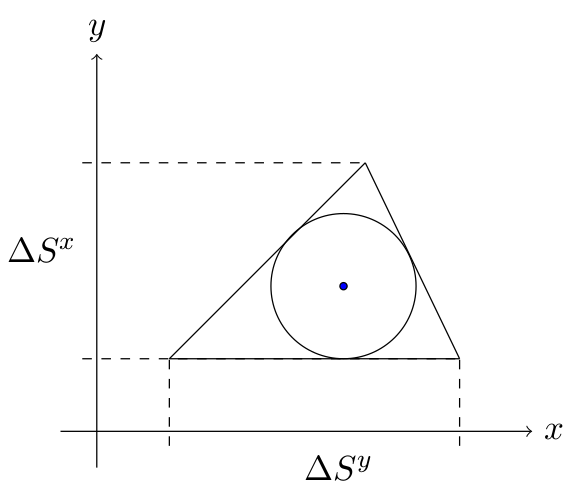
\includegraphics[width = \textwidth]{Zeitdiskretisierung.png}
		\end{figure}
	\end{columns}

\end{frame}

%------------------------------------------------
\section{Ergebnisse}

\subsection{SineWave Testcase}


\begin{frame}
	\frametitle{SineWave Testcase}
	\framesubtitle{Konvergenzordnung}
	Es wird ein sinusförmiger Dichtepuls transporiert.
	
\begin{columns}
	
	\column{0.55 \textwidth}
	Raumordnung: \quad 1, 2\\
	$\mu$: \quad \quad \quad \quad \quad \quad \quad 0, 0.01, 0.05, 0.1\\
	Gitterzahl: \quad \quad \quad 100x100, 200x200, 400x400
	\vspace*{0.5cm}


	Die empirische Konvergenzordnung des Verfahrens ergibt sich zu
	\begin{equation}
		n=\frac{log(\frac{E_1}{E_2})}{log(\frac{h_1}{h_2})},
	\end{equation}
	
	wobei E die Diskretisierungsfehler und h den gemittelten Gitterabstand darstellen.
	% variiert wurden hier 1. Ordnung, 2. mu 3. Gitter
	% Ausführliche Ergebnisse im Anhang
	%

	\column{0.4 \textwidth}
	\vspace*{-2cm}
	\begin{figure}
		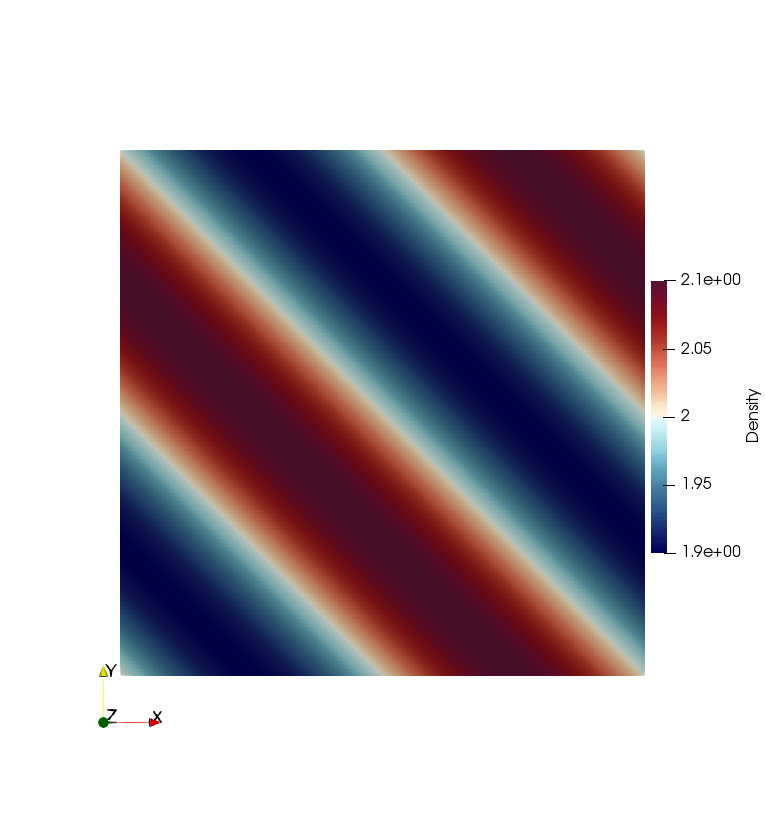
\includegraphics[width=\textwidth]{sinus_wave_density.png}
		\vspace*{-1cm}
		\caption{SineWave Testcase Density für $\mu=0.1$}
	\end{figure}
\end{columns}
\end{frame}




% \begin{frame}
% 	\frametitle{SineWave Testcase}

% 	\begin{figure}
% 		\includegraphics[width=0.8\linewidth]{SineWave_viscous.png}
% 		\caption{SineWave Testcase VelocityMagnitude für $\mu=0.2$ und $t=0.1s$, sowie $t=2.5s$}
% 	\end{figure}
% 	% hier konnte optisch kein Unterschied gesehen werden bei verschiedenen Viskositäten, hier aber der Vergleich nach t=0.1s und t=2.5s
% 	% Interessant: Die Farben werden intensiver, also größere/kleinere Werte! Hätte ich anders erwartet.

% \end{frame}



\begin{frame}
	\frametitle{SineWave Testcase}
	\framesubtitle{Konvergenzordnung}

		\begin{table}
			\begin{tabular}{l l l l l}
				\toprule
				Ordnung & $\mu$  & $n_2$-Ordnung & Rechenzeit [s]\\
				\midrule
				1 (E) & - & 0.983 & 68.11\\
				1 (NS) & 0 & 0.980 & 91.50\\
				1 (NS) & 0.01  & 0.979& 387.41\\
				1 (NS) & 0.05 &  0.962 & 1906.77\\
				1 (NS) & 0.1 &  0.972  & 3263.09\\
				\bottomrule
			\end{tabular}
			\caption{Rechenzeit (400x400 Zellen) und Ordnung bei O1. }
	\end{table}

% Euler war im Prinzip gleich wie NS mu=0
%Frage: Warum entspricht die empirische Konvergenzordnung nicht 1 bzw 2? Warum ist die geringer?
%Frage: für O1 werden die Ableitungen hier mit den integralen Zellmittelwerten gebildet (eigentlich Entkopplung?)

\end{frame}



\begin{frame}
	\frametitle{SineWave Testcase}
	\framesubtitle{Konvergenzordnung}

		\begin{table}
			\begin{tabular}{l l l l l}
				\toprule
				Ordnung & $\mu$  & $n_2$-Ordnung & Rechenzeit [s]\\
				\midrule
				2 (E) & - & 1.84 & 300.55\\
				2 (NS) & 0 &  1.85 &262.63 \\
				2 (NS) & 0.01 &2.02 &1205.84 \\
				2 (NS) & 0.05  & 1.87& 6123.78 \\
				2 (NS) & 0.1 &  1.81& 11998.56\\
				\bottomrule
			\end{tabular}
			\caption{Rechenzeit (400x400 Zellen) und Ordnung bei O2. }
	\end{table}

% Euler war im Prinzip gleich wie NS mu=0
%Frage: Warum entspricht die empirische Konvergenzordnung nicht 1 bzw 2? Warum ist die geringer?
%Frage: für O1 werden die Ableitungen hier mit den integralen Zellmittelwerten gebildet (eigentlich Entkopplung?)

\end{frame}


	% \begin{frame}
	% 	\frametitle{SineWave Testcase}
	% 	\framesubtitle{Konvergenzordnung}
	
	% 	\begin{tabular}{|c|c|c|c|c|}
	% 		\hline
	% 		Ordnung & $\mu$  & $n_1-Ordnung$& $n_2-Ordnug$& $n_{inf}-Ordnung$\\

	% 		2 & 0 &  1.85  \\
	% 		2 & 0.01 &2.02  \\
	% 		2 & 0.05  & 1.87  \\
	% 		2 & 0.1 &  1.81 \\
	% 		\end{tabular}
	
	% % Euler war im Prinzip gleich wie NS mu=0
	% %Frage: Warum entspricht die empirische Konvergenzordnung nicht 1 bzw 2? Warum ist die geringer?
	% %Frage: für O1 werden die Ableitungen hier mit den integralen Zellmittelwerten gebildet (eigentlich Entkopplung?)
	
	% 	\end{frame}






% \begin{frame}
% 	\frametitle{SineWave Testcase}
% 	\framesubtitle{Rechenzeit}
% 	\begin{table}[h]
% 	\begin{tabular*}{0.4\textwidth}{|c|c|c|c|}
% 		\hline
% 		O & $\mu$ & Gitter & Rechenzeit [s]\\
% 		\hline
% 		1 & 0 & 100x100 & 1.99\\
% 		\hline
% 		1 & 0.01 & 100x100 & 1.46\\
% 		\hline
% 		1 & 0.05 & 100x100 & 6.67\\
% 		\hline
% 		1 & 0.1 & 100x100 & 14.0\\
% 		\hline
% 		1 & 0 & 200x200 & 10.18\\
% 		\hline
% 		1 & 0.01 & 200x200 & 21.99\\
% 		\hline
% 		1 & 0.05 & 200x200 & 102.76\\
% 		\hline
% 		1 & 0.1 & 200x200 & 226.78\\
% 		\hline
% 		1 & 0 & 400x400 & 91.5\\
% 		\hline
% 		1 & 0.01 & 400x1400 & 387.41\\
% 		\hline
% 		1 & 0.05 & 1400x400 & 1906.77\\
% 		\hline
% 		1 & 0.1 & 400x1400 & 3263.09\\
% 		\hline
% 	\end{tabular*}
% 	\hspace{0.05\textwidth}
% 	\begin{tabular*}{0.4\textwidth}{@{\extracolsep{\fill}}|c|c|c|c|}
% 		\hline
% 		O & $\mu$ & Gitter & Rechenzeit [s]\\
% 		\hline
% 		2 & 0 & 100x100 & 4.74\\
% 		\hline
% 		2 & 0.01 & 100x100 & 4.93\\
% 		\hline
% 		2 & 0.05 & 100x100 & 24.55\\
% 		\hline
% 		2 & 0.1 & 100x100 & 46.84\\
% 		\hline
% 		2 & 0 & 200x200 & 33.05\\
% 		\hline
% 		2 & 0.01 & 200x200 & 74.19\\
% 		\hline
% 		2 & 0.05 & 200x200 & 368.89\\
% 		\hline
% 		2 & 0.1 & 200x200 & 737.04\\
% 		\hline
% 		2 & 0 & 400s400 & 262.63 \\
% 		\hline
% 		2 & 0 & 400s400 & 1205.84 \\
% 		\hline
% 		2 & 0 & 400s400 & 6123.78 \\
% 		\hline
% 		2 & 0 & 400s400 & 11998.56 \\
% 		\hline
% 		\end{tabular*}
% 	\end{table}

%learnings 1. teilweise ist die ns mit geringem mu schneller als euler?!
%          2. Rechenzeit steigt wie zu erwarten mit der Gitteranzahl
%          3. Rechenzeit steigt mit mu um den faktor mu (DFL-Bedingung)
% \end{frame}

\subsection{Blasius Boundary Layer}
\begin{frame}
	\frametitle{Blasius Grenzschicht}
	
	\begin{columns}
	\column{0.6\textwidth}

		\begin{itemize}
			\item Entdimensionalisierung der Größen
			\item Vergleich der numerischen Ergebnisse mit der analytischen Lösung der Grenzschichtgleichung.
			\item Implizite Berechnung (DFL-Bedingung)
		\end{itemize}
	\column{0.3\textwidth}
	Grenzschichtgleichung:
	\begin{equation}
		\delta_{99} = \frac{5 \cdot x}{\sqrt{Re_x}}
	\end{equation}
	\end{columns}
	



	\begin{center}
		\begin{figure}
			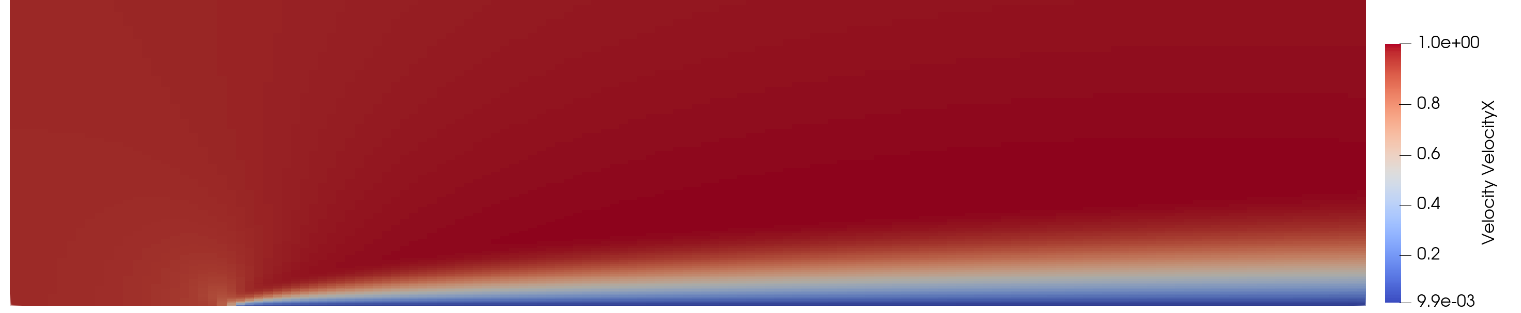
\includegraphics[width=0.9\linewidth]{boundary_layer.png}
			\caption{Axialgeschwindigkeit über einer laminar angeströmten ebenen Platte.}
		\end{figure}
	\end{center}
\end{frame}

\begin{frame}
	\frametitle{Grenzschichtströmung}
	\framesubtitle{Geschwindigkeitsprofil}
	\begin{center}
		\begin{figure}
			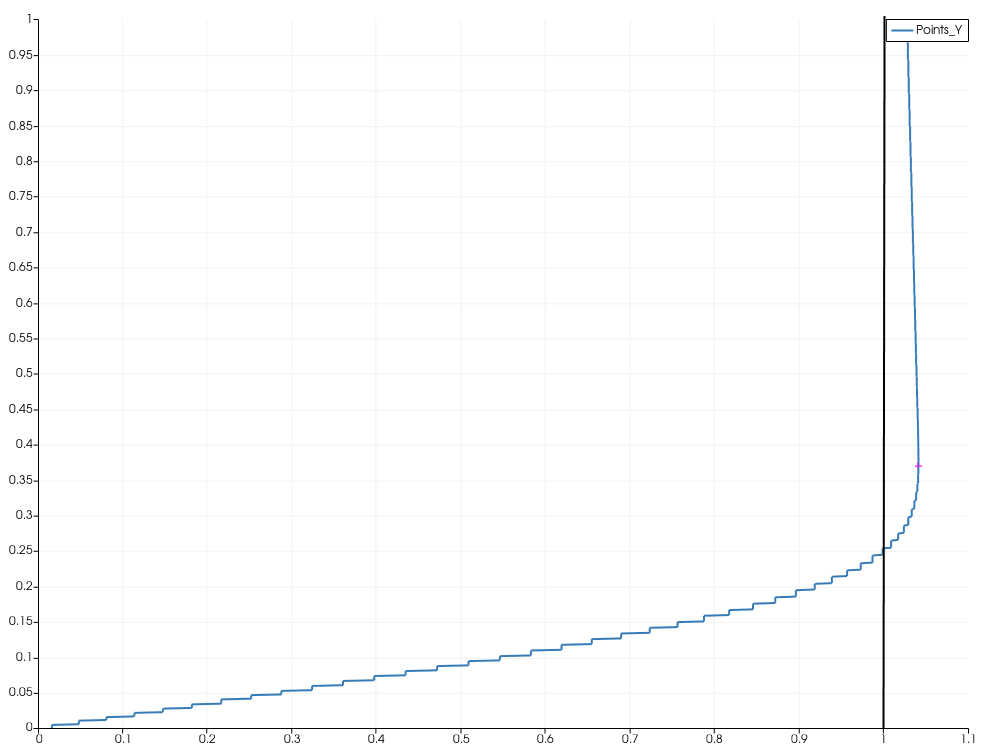
\includegraphics[width=0.5\linewidth]{vx_x=2.2.png}
			\caption{Profil der Axialgeschwindigkeit an der Stelle x=2.}
		\end{figure}
	\end{center}
% Warum ist v>1 teils? -> Masseerhaltung
\end{frame}

\begin{frame}
	\frametitle{Grenzschichtströmung}
	\framesubtitle{Grenzschichtdicke}
	\begin{center}
		\begin{figure}
			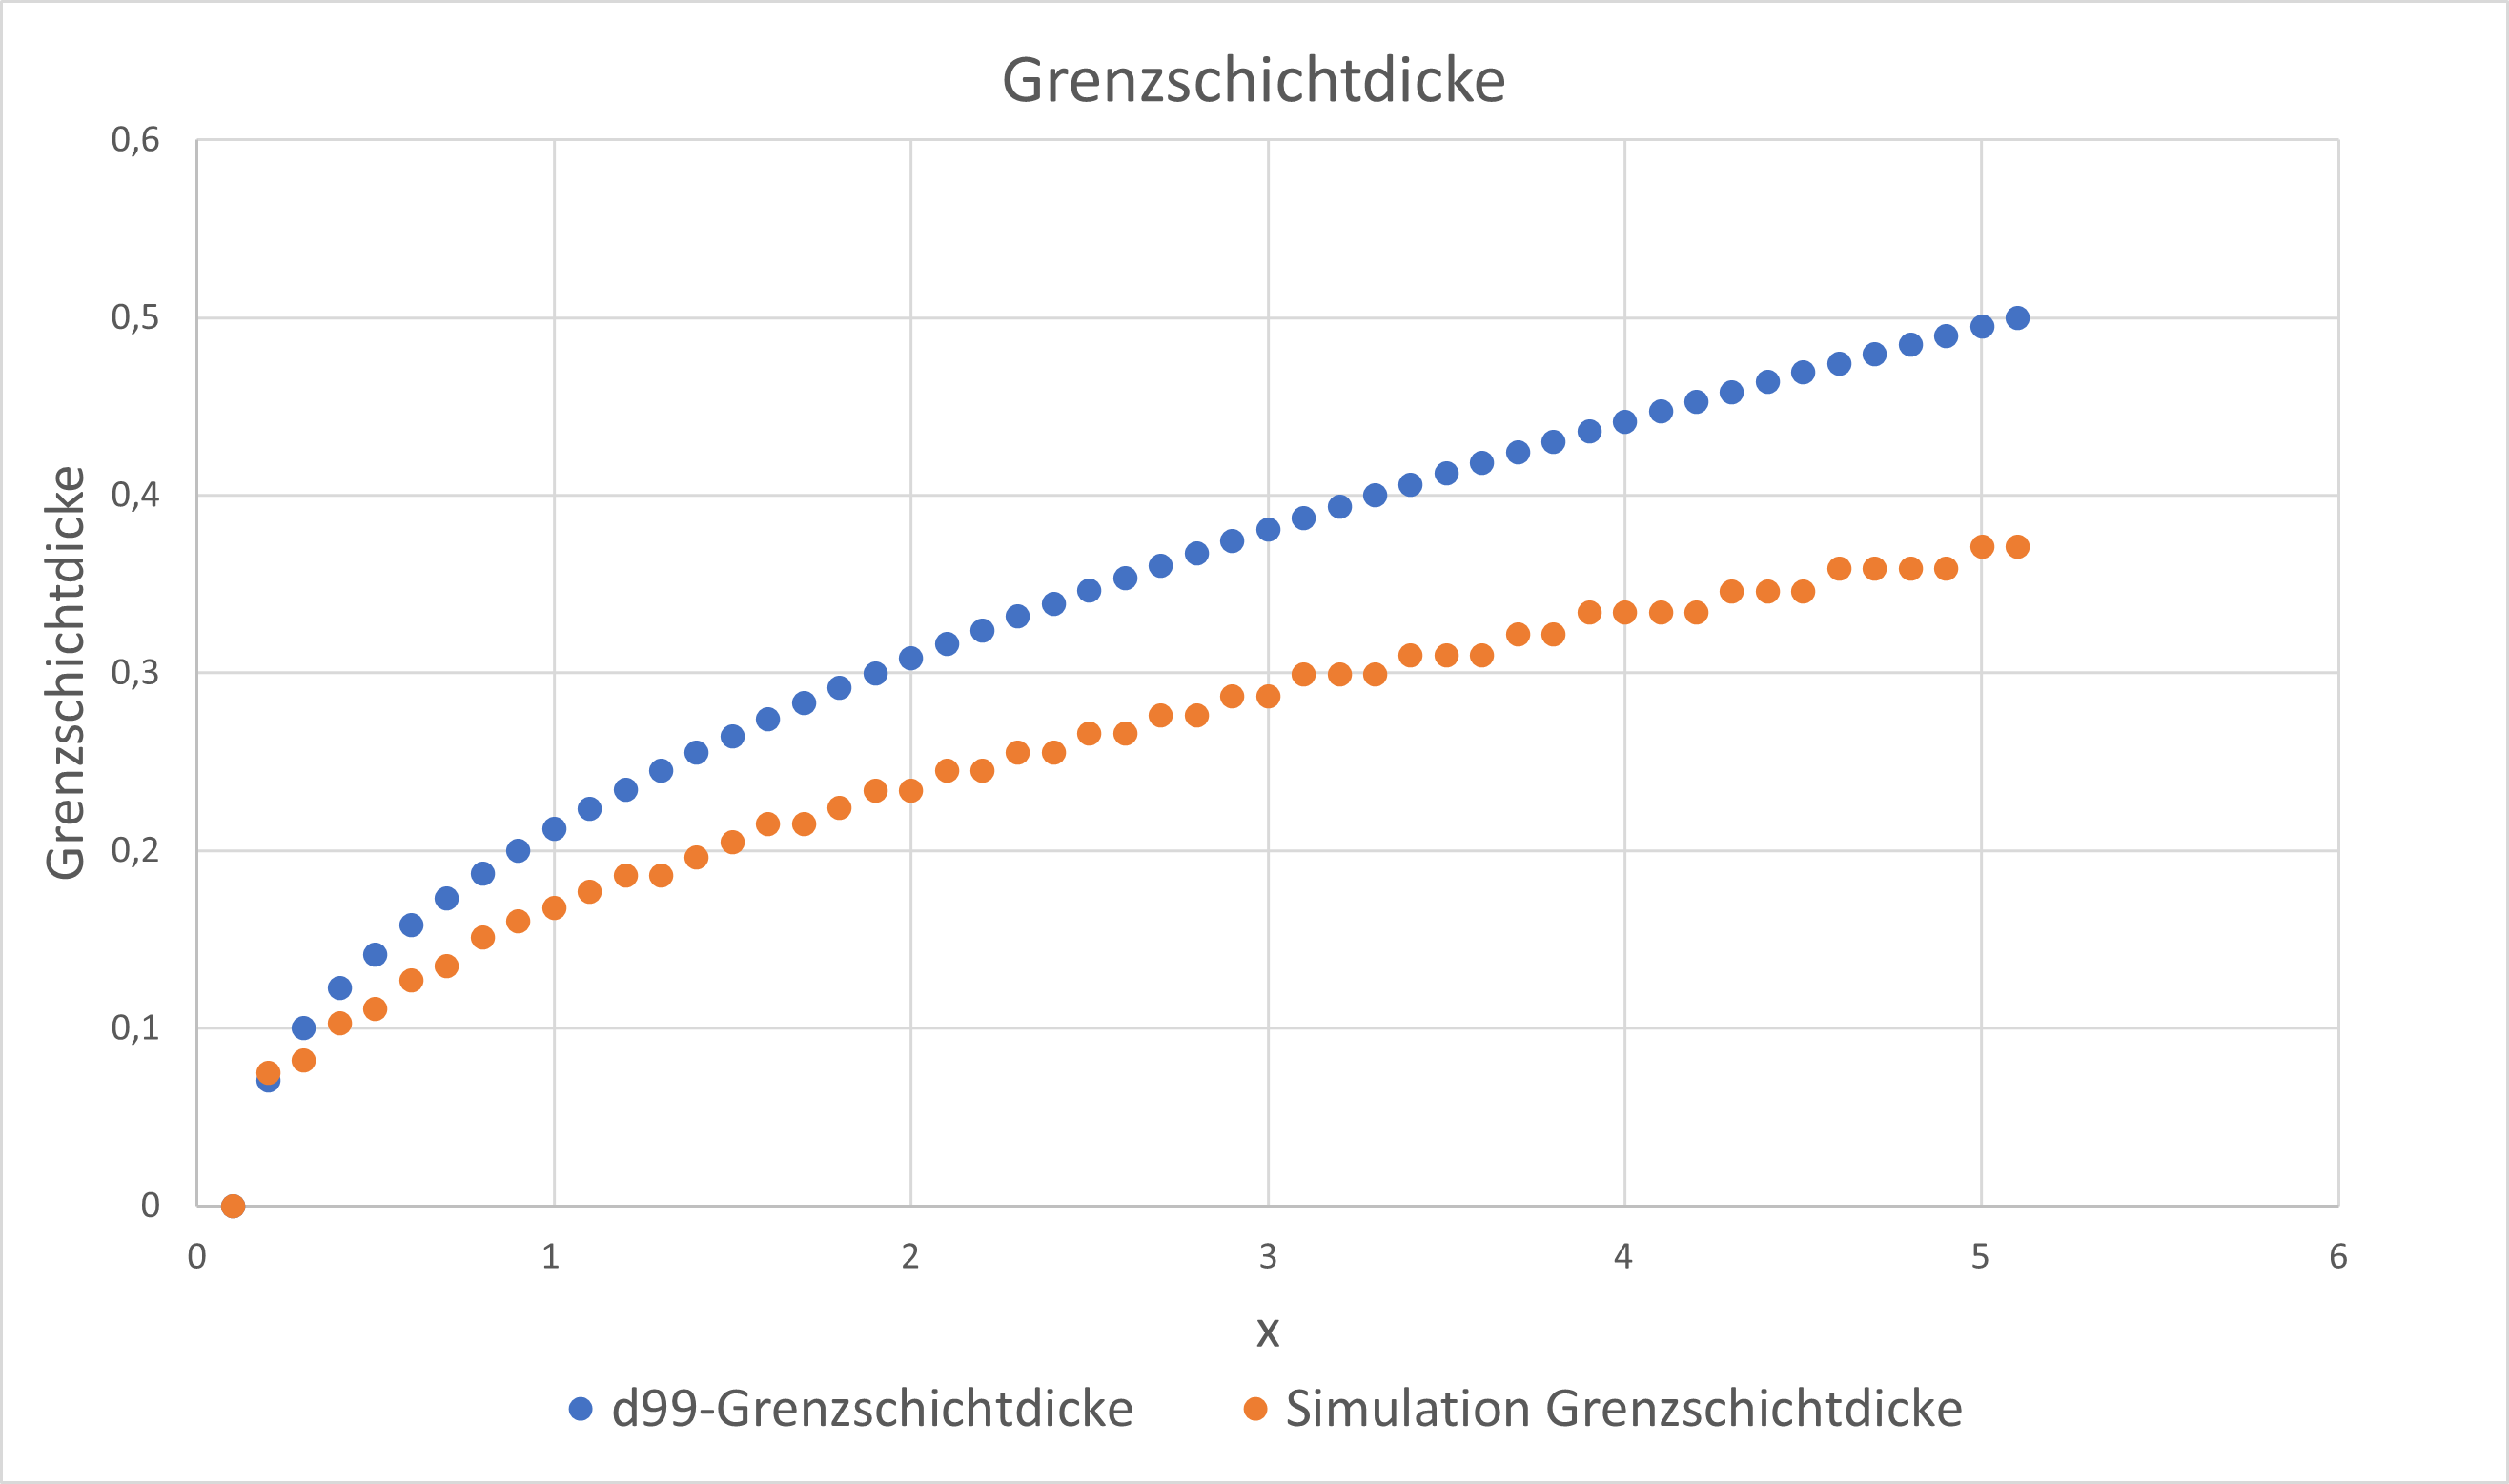
\includegraphics[width=0.6\linewidth]{a2_plot.png}
			\caption{Vergleich der theoretischen Grenzschichtdicke zur Simulation.}
		\end{figure}
	\end{center}
% relativ gute Übereinstimmung. 
% Warum wird hier implizit gerechnet??
% Warum wird GS nicht turublent? -> Weil wir 2D sind! (Außerdem Re-Zahlen viel zu gering, am Ende Re=2500 (Re_krit = 5*10^5))
\end{frame}


\subsection{Zylinderumströmung}
\begin{frame}
\frametitle{Cylinder Testcase}
\framesubtitle{Viskoser Fall oben - Euler Fall unten}
\vspace*{-0.2cm}
\begin{figure}
	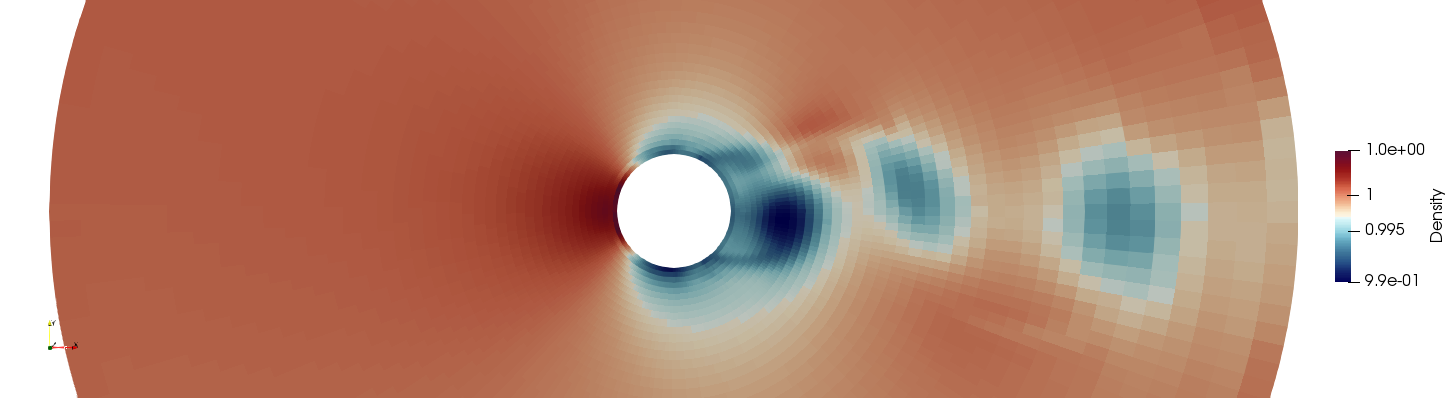
\includegraphics[width=0.8\linewidth]{Cylinder_Wirbelstrasse.png}
	%\caption{Cylinder Testcase ohne Reibungseinfluss (links) und mit Reibungseinfluss (rechts)}
%Auffallend: 1. Karmansche Wirbelstraße 
\end{figure}
\vspace*{-0.5cm}
\begin{figure}
	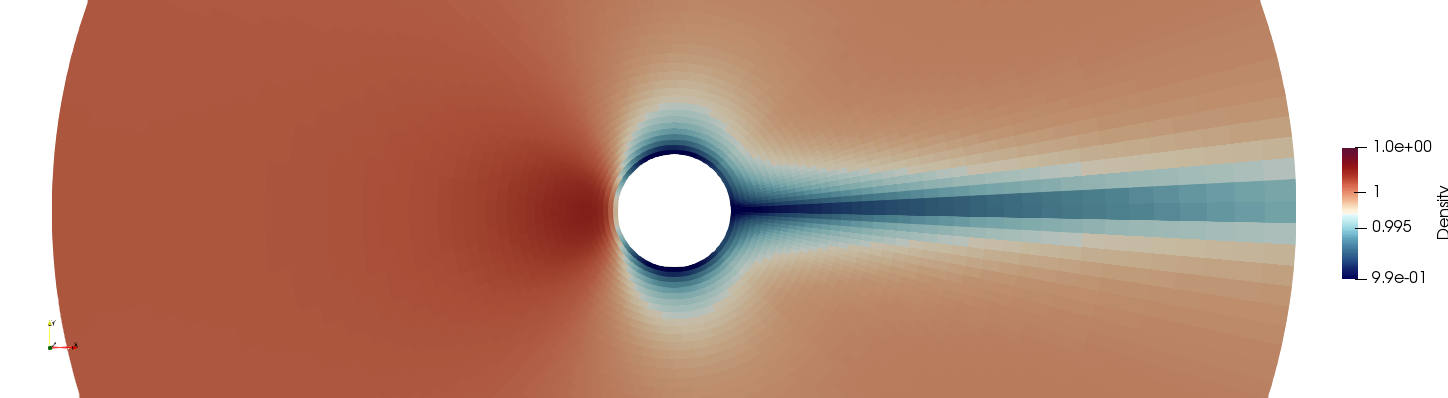
\includegraphics[width=0.8\linewidth]{Cylinder_euler_1.png}
	%\caption{Cylinder Testcase ohne Reibungseinfluss (links) und mit Reibungseinfluss (rechts)}
%Auffallend: 1. Karmansche Wirbelstraße 
\end{figure}

%Bild Euler vs. NS

% Phänomene erklren

\end{frame}
\begin{frame}
	\frametitle{Cylinder Testcase}
	\framesubtitle{Auftriebs- und Widerstandsbeiwert}

	\begin{figure}
		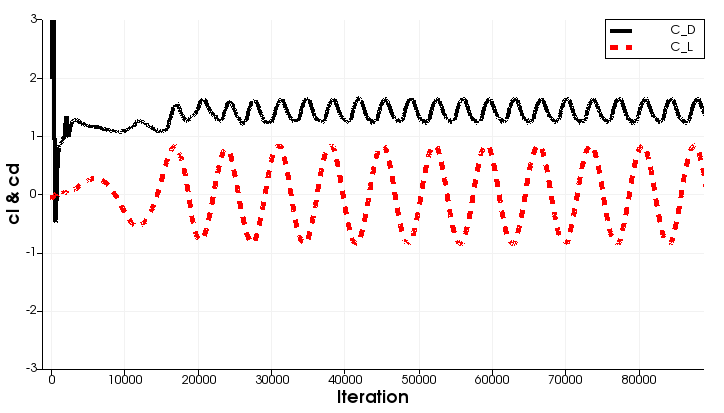
\includegraphics[width=0.8\linewidth]{CL_CD.png}
		%\caption{Verlauf des Auftriebs- und Widerstandbeiwertes über der Iteration für $\mu=0.002$}
	\end{figure}


	\begin{table}
		\begin{tabular}{l l l l l}
			\toprule
			Rechnung & Rechenzeit [s]& $c_l [-]$  & $c_d [-]$\\
			\midrule
			$\mu = 0$ & 150.83 & 0.001063 & 0.323603\\
			$\mu = 0.001$& 3229.61 & [-0.8; 0.8] & [0.8; 1.2]\\
			\bottomrule
		\end{tabular}
		\caption{Rechenzeit und Ordnung bei O1}
	\end{table}
% Reibung ist jetzt dabei -> Reibungswiderstand
% führt zu instationärer Strömung -> Karmansche Wirbelstraße
% Wirbel erzeugen durch Zirkulationserhaltung Auftrieb
\end{frame}


\begin{frame}
	\frametitle{Cylinder Testcase}
	\framesubtitle{Vergleich Auftriebs- und Widerstandsbeiwert}

	\begin{table}
		\begin{tabular}{l l l l l}
			\toprule
			Rechnung & Rechenzeit [s]& $c_l [-]$  & $c_d [-]$\\
			\midrule
			$\mu = 0$ & 150.83 & 0.001063 & 0.323603\\
			$\mu = 0.002$& 3229.61 & [-0.8; 0.8] & [1.259; 1.63]\\
			\bottomrule
		\end{tabular}
		%\caption{Rechenzeit und Ordnung bei O1}
	\end{table}
% Reibung ist jetzt dabei -> Reibungswiderstand
% führt zu instationärer Strömung -> Karmansche Wirbelstraße
% Wirbel erzeugen durch Zirkulationserhaltung Auftrieb
\end{frame}



%------------------------------------------------

%Schlussfolie

%------------------------------------------------
 \section{Lessons learned}

 \begin{frame}
 	\frametitle{Lessons learned}

	\begin{itemize}
		\item DFL-Bedingung erhöht Rechenzeit unter Umständen spürbar
		\item Viskosität hat keinen Einfluss auf das Konvergenzverhalten
		\item Ergebnisse der numerischen Lösung sind Modellabhängig $\Rightarrow$ Vorsicht bei der Konstruktion der Randbedingungen! 
	\end{itemize}

 \end{frame}


%----------------------------------------------------------------------------------------
%	CLOSING SLIDE
%----------------------------------------------------------------------------------------

\begin{frame} % The optional argument 'plain' hides the headline and footline
	 	\begin{center}
		
		\bigskip \bigskip % Vertical whitespace
		
		{\Large Vielen Dank für die Aufmerksamkeit!}
		\begin{figure}
			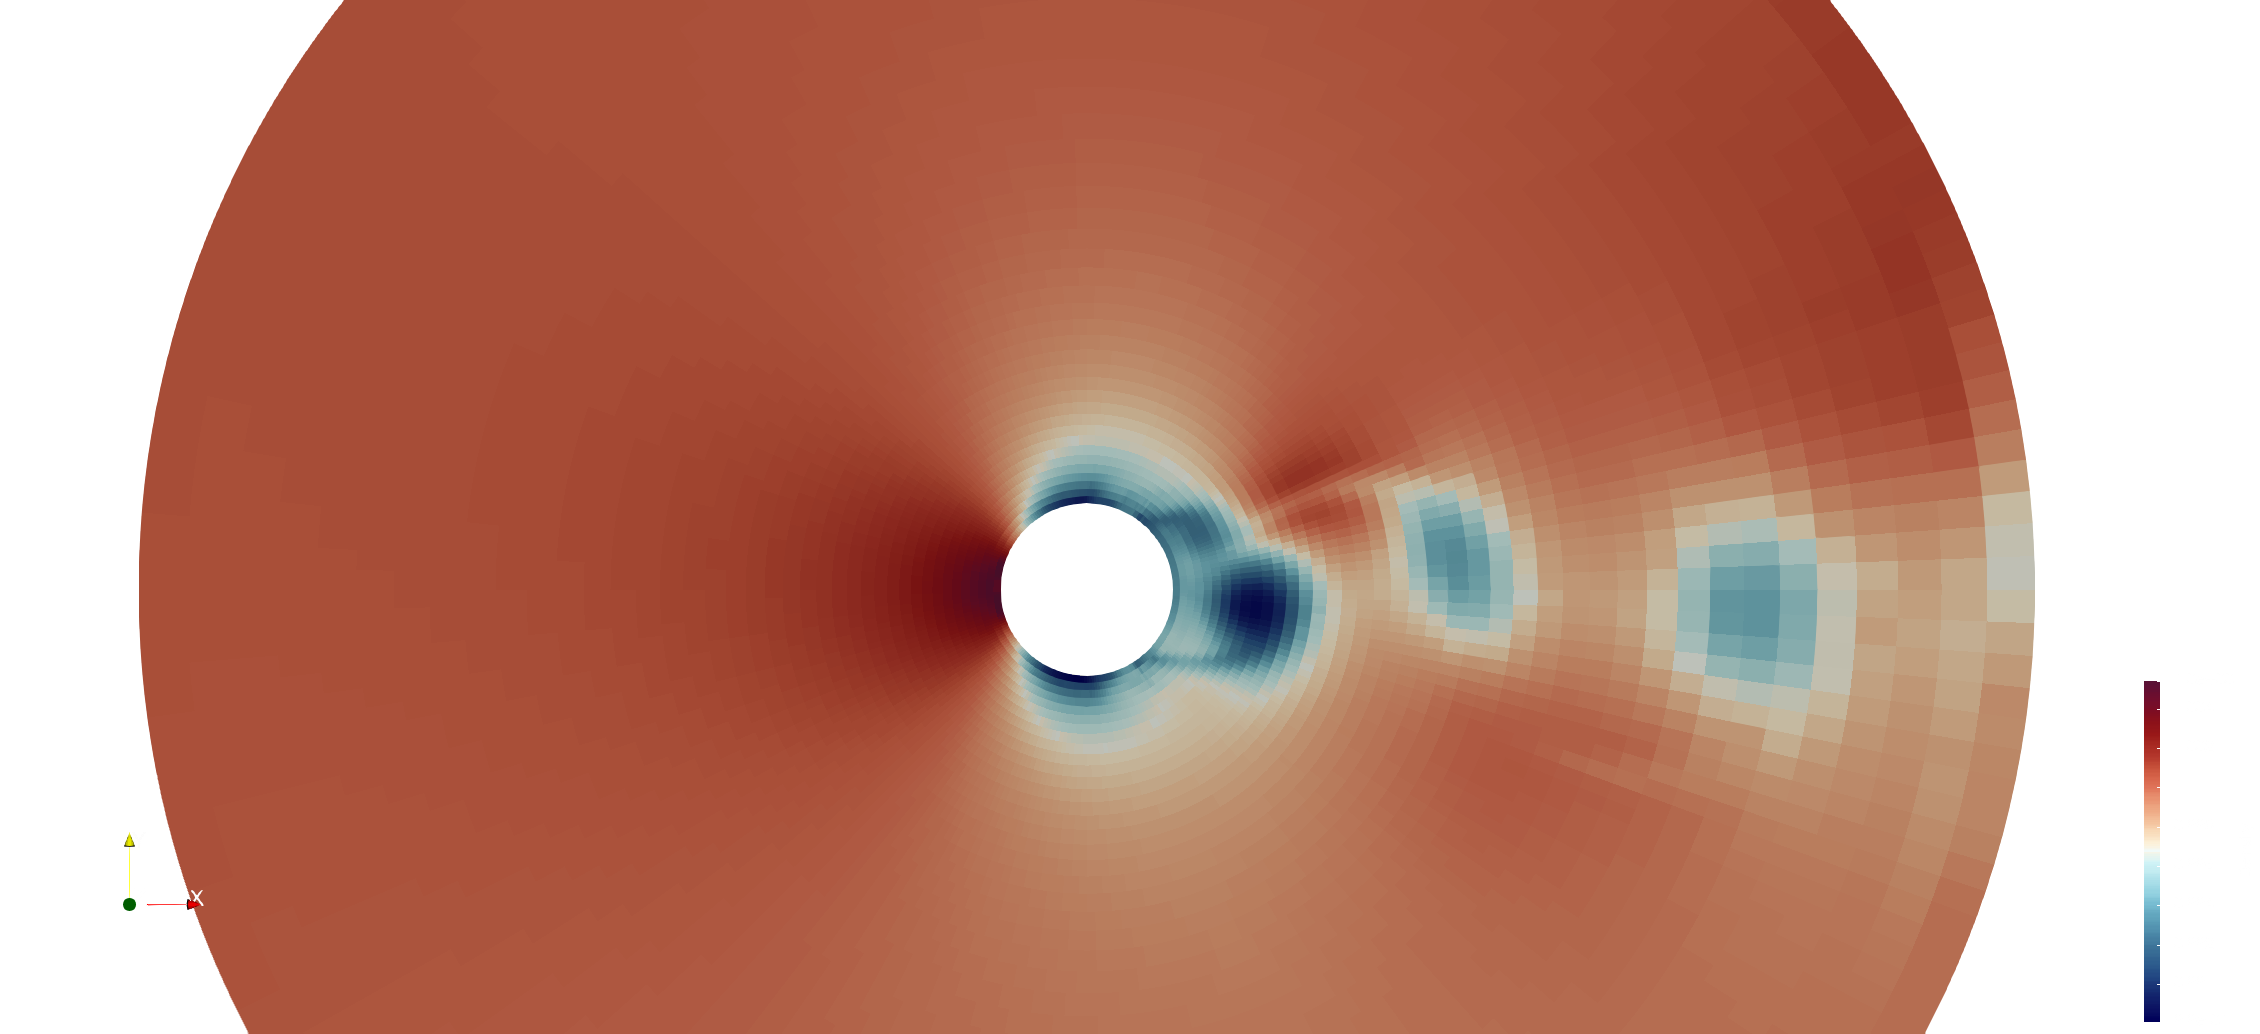
\includegraphics[width=0.5\linewidth]{Navier.png}
			%\caption{Gausspuls auf kartesischem Gitter (oben) und unstrukturiertem kreisförmigem Gitter (unten)}
		\end{figure}
	\end{center}
 \end{frame}

%----------------------------------------------------------------------------------------\begin{frame}[plain] % The optional argument 'plain' hides the headline and footline


	\begin{frame}
		\frametitle{Anhang}
		\subtitle{Daten A1}
	
		\begin{tabular}{|c|c|c|c|c|c|}
			\hline
			Ordnung & $\mu$ & Gitter & $L_1-Fehler$& $L_2-Fehler$& $L_{inf}-Fehler$\\
			\hline
			1 & 0 & 100x100 & 3.36E-3 & 4.26E-3 & 1.11E-2 \\
			\hline
			1 & 0 &200x200 &1.71E-3 & 2.17E-3 & 5.73E-3 \\
			\hline
			1 & 0 &400x400 &8.67E-4 & 1.10E-3 & 2.93E-3 \\
			\hline
			2 & 0 &100x100 &7.97E-5 & 1.13E-4 & 5.16E-4 \\
			\hline
			2 & 0 &200x200 &2.04E-5 & 2.80E- & 1.42E-4\\
			\hline
			2 & 0 &400x400 &5.86E-6 & 7.78E-6 & 4.05E-5 \\
			\hline
			1 & 0.01 &100x100 & 3.19E-3& 4.06E-3 & 1.06E-2 \\
			\hline
			1 & 0.01 &200x200 & 1.59E-3& 2.01E-3 & 6.55E-3 \\
			\hline
			1 & 0.01 &400x400 & 8.15E-4 & 1.02E-3 & 3.89E-3 \\
			\hline
			2 & 0.01 &100x100 & 5.26E-5& 6.79E-5 & 2.61E-4 \\
			\hline
			2 & 0.01 &200x200 & 1.25E-5& 1.62E-5 & 7.32E-5 \\
			\hline
			2 & 0.01 &400x400 & 3.06E-6& 4.00E-6 & 2.23E-5 \\
			\hline
			\end{tabular}
		\end{frame}
	
	
	\begin{frame}
		\frametitle{Flussberechnung auf strukturierten Gittern}
		%Satz von Green liefert Zusammenhang zwischen Volumen- und Oberflächenintegral
		1. Satz von Green
		$$\int_{v'} \frac{\partial f}{\partial x} - \frac{\partial g}{\partial y}\,dx =  \oint_{\partial v'} g dx + f dy$$
		2. Setze $f = u; g = 0$\\
		3. Integral auflösen
		$$V'\frac{\partial u}{\partial x} = \vartriangle y (U_{i,j} + U_{i+1,j})$$
		$$ \Rightarrow \frac{\partial u}{\partial x} = \frac{U_{i,j} + U_{i+1,j}}{\vartriangle  x}$$
		Analog:
		$$\frac{\partial u}{\partial y} = \frac{U_{i+\frac{1}{2},j+\frac{1}{2}}+ U_{i+\frac{1}{2},j-\frac{1}{2}}}{\vartriangle y}$$
		
	\end{frame}
	
	%---------------------------------------------
	\subsection{Flussberechnung}
	
	
	\begin{frame}
		\frametitle{Flussbrechung auf strukturierten Gittern}
		\begin{columns}
			
			\column{0.45\textwidth}
			Bei der Gradientenbestimmung werden Werte an den Seitenmittelpunkten verwendet.
			Diese werden wie folgt berechnet:
			$$U_{i+\frac{1}{2}, j + \frac{1}{2}} = \frac{1}{4} (U_{i,j}+U_{i,j+1}+U_{i+1,j}+U_{i+1,j+1}) $$
			$$U_{i+\frac{1}{2}, j + \frac{1}{2}} = \frac{1}{4} (U_{i,j}+U_{i,j+1}+U_{i+1,j}+U_{i+1,j+1})$$
			\column{0.45\textwidth}
			
			\begin{figure}
				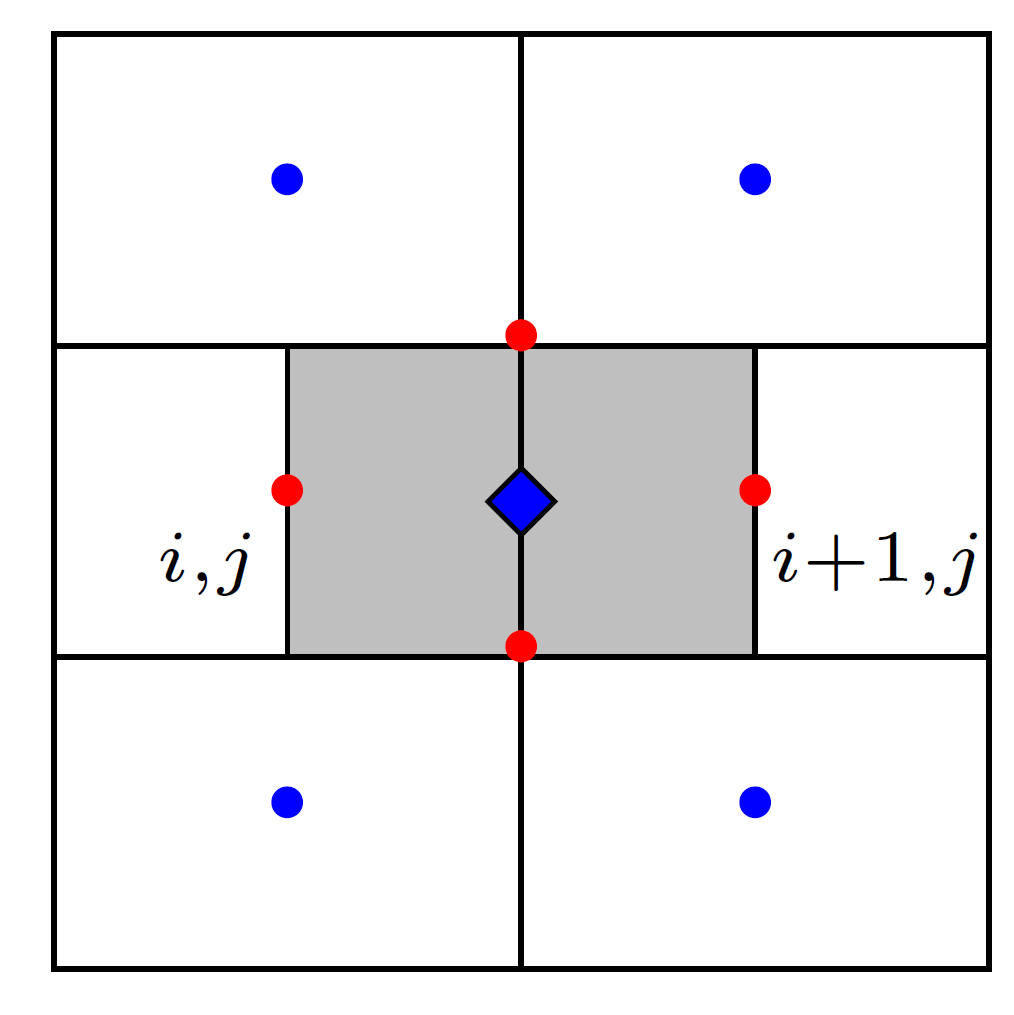
\includegraphics[width=0.7\linewidth]{Mittellung_ueber_Zellen.png}
			\end{figure}
		\end{columns}
	\end{frame}
	
	\begin{frame}
		\frametitle{Flussberechnung auf unstrukturierten Gittern}
		Im Gegensatz zum strukturierten Gitter müssen auf unstrukturierten Gittern auch die nicht abgeleiteten Größen
		durch Mittelung der Nachbarzellen bestimmt werden.
		\begin{columns}
			\column{0.45\textwidth}
			\begin{figure}
				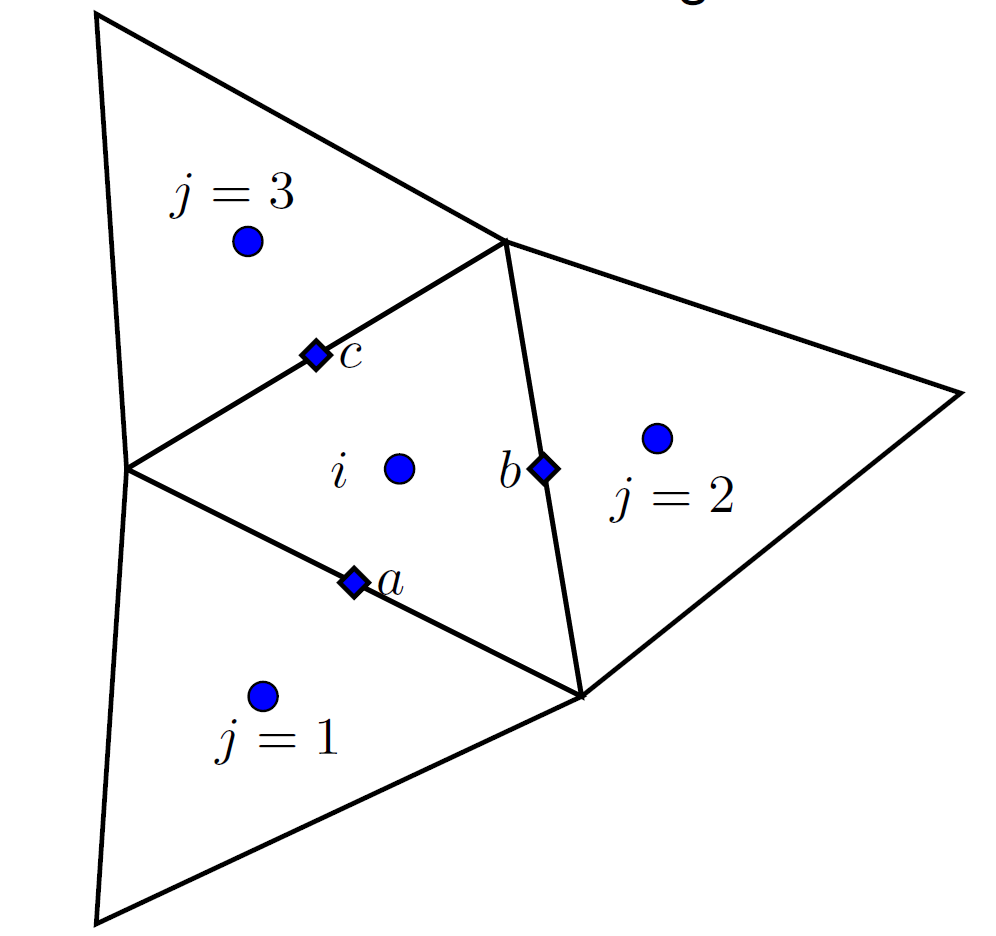
\includegraphics[width=0.8\linewidth]{unstruct_flux.png}
			\end{figure}
			
			
			\column{0.45\textwidth}
			\begin{align}
			(v_1)_a &= \frac{(v_1)_{i,a}+(v_1)_{j,a}}{2} \\
			(v_2)_a &= \frac{(v_2)_{i,a}+(v_2)_{j,a}}{2} \\
			(\mu_2)_a &= \frac{(\mu)_{i,a}+(\mu)_{j,a}}{2} \\
			(\lambda)_a &= \frac{(\lambda)_{i,a}+(\lambda)_{j,a}}{2}
			\end{align}
		\end{columns}
		
	\end{frame}	
	
	
	\begin{frame}
		\frametitle{Flussberechnung auf unstrukturierten Gittern}
		Die Gradienten können auf den Zellseiten nicht effizient mit dem Satz von Green bestimmt werden.
		Lösung mit dem empirischen Ansatz:
		
		\begin{equation}
		\nabla U_a = (\overline{\nabla U})_{i,j} - \biggl\lbrack(\overline{\nabla U})_{i,j} \cdot 
		\vec{t_{i,j}}- \biggl(\frac{\partial U }{\partial l}\biggr)_{i,j}  \biggr\rbrack \vec{t_{i,j}}
		\end{equation}
		
		
		Dabei ist $\vec{t_{i,j}} = \frac{\vec{r}_{i,j}}{l_{i,j}}$ der Vektor, zu dem der Gradient
		\begin{equation}
		(\overline{\nabla U})_{i,j} = 0.5 (\nabla U_i+\nabla U_j)
		\end{equation}
		verwendet wird. Tangential zu $\vec{t_{i,j}}$ wird die Richtungsableitung 
		
		\begin{equation}
		\biggl(\frac{\partial U }{\partial l}\biggr)_{i,j} = \frac{U_j-U_i}{l_{i,j}}
		\end{equation}
		verwendet.
		
	\end{frame}
	
	
	
	
	
	
	\begin{frame}
		\frametitle{Anhang}
		\subtitle{Daten A1}
		\begin{tabular}{|c|c|c|c|c|c|}
			\hline
			Ordnung & $\mu$ & Gitter & $L_1-Fehler$& $L_2-Fehler$& $L_{inf}-Fehler$\\
			\hline
			1 & 0.5 &100x100 & 2.98E-3& 3.72E-3 & 1.23E-2 \\
			\hline
			1 & 0.5 &200x200 & 1.55E-3& 1.93E-3 &7.00E-3  \\
			\hline
			1 & 0.05 &400x400 &7.94E-4 & 9.91E-4 & 3.84E-3 \\
			\hline
			2 & 0.05 &100x100 & 5.08E-5& 7.10E-5 & 3.32E-4 \\
			\hline
			2 & 0.05 &200x200 & 1.28E-5& 1.90E-5 & 1.16E-4 \\
			\hline
			2 & 0.05 &400x400 &3.27E-6 & 5.20E-6 & 4.07E-5 \\
			\hline
			1 & 0.1 &100x100 &3.22E-3 & 3.90E-3 & 1.21E-2 \\
			\hline
			1 & 0.1 &200x200 & 1.67E-3& 2.02E-3 & 6.73E-3 \\
			\hline
			1 & 0.1 &400x400 & 8.53E-4& 1.03E-3 & 3.58E-3 \\
			\hline
			2 & 0.1 &100x100 & 5.58E-5& 8.57E-5 & 4.18E-4 \\
			\hline
			2 & 0.1 &200x200 & 1.44E-5& 2.42E-5 & 1.52E-4 \\
			\hline
			2 & 0.1 &400x400 & 3.70E-6& 6.88E-6 & 5.56E-5 \\
			\hline
			\end{tabular}
			
	
	% Tabelle mit den empirischen Konvergenzordnungen
	% Unterschied L1,L2,Linf erklären
	
	\end{frame}

	\begin{frame}
		\frametitle{Blasius-Gleichung}

		Die Blasius-Gleichung ist eine Vereinfachung der Navier-Stokes Gleichungen und beschreibt die stationäre, inkompressible Strömung auf einer 2D Ebenen Platte auf der sich eine Grenzschicht ausbildet.
		$$f''(\theta)+\frac{1}{2} \\ f'(\theta)\cdot\int_{0}^{\theta} f(t) \,dt $$
	\end{frame}

\end{document} 